\documentclass[12pt, letterpaper]{article}
\usepackage{import}
\usepackage[margin=0.5in]{geometry}
\usepackage{graphics}
\usepackage{xcolor}
\usepackage{bbm}
\usepackage[charter]{mathdesign}
\usepackage[hidelinks]{hyperref}


\graphicspath{{images/}}

\import{./preambule}{/python_highlights.tex}
\import{./preambule}{/polish.tex}
\import{./preambule}{/math_preambule.tex}
\import{./preambule}{/macros.tex}

\title{
    \huge Podstawy Sterowania Optymalnego\\Labolatorium 4\\
    \large Regulator PID - Optymalizacja układów liniowych.
}
\author{Prowadzący: mgr inż. Krzysztof Hałas\\
        Wykonał: Ryszard Napierała}
\date{\today}

\begin{document}
    \maketitle
    
    \section*{Zadanie 5}
        \begin{figure}[H]
            \centering
            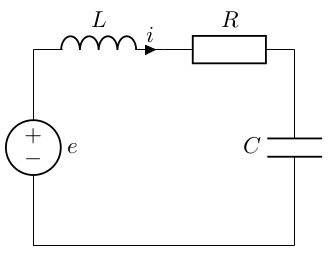
\includegraphics[width=0.5\textwidth]{lab4/rys1}
            \caption{Układ RLC}
            \label{fig:rlc}
        \end{figure}

        \begin{enumerate}
            \itemcl[]{W języku Python zaimportować biblioteki \emph{numpy, scipy.signal,\\
                scipy.itegrate.solve\_ivp, scipy.integrate.odeint}, a następnie \emph{matplotlib.pyplot}}{lab4.py}{2}{4}

            \itemcl[]{Wprowadzić zmienne regulatora PID $K_p=2$, $T_I=1$, $T_D=4$ oraz
                parametry obiektu z rysunku \ref{fig:rlc}.}{lab4.py}{8}{21}
                \outputTxt{snippets/lab4/zad5_1.txt}

            \itemcl[
                \[G_{PID}=K_p(1+\frac{1}{sT_I}+sT_D)=
                    \frac{K_pT_Ds^2+K_ps+\frac{K_p}{T_I}}{s}\]
                \[G_o=\frac{5}{s^3+9s^2+27s+27}\]
                \[G_u=G_{PID}*G_o\]
                \[G_u=\frac{5(K_pT_Ds^2+K_ps+\frac{K_p}{T_I})}
                    {s(s^3+9s^2+27s+27)}=
                    \frac{5K_pT_Ds^2+5K_ps+\frac{5K_p}{T_I}}
                    {s^4+9s^3+27s^2+27s}\]
                \[G_z=\frac{G_u}{1+G_u}\]
                \[G_z=\frac{\frac{5K_pT_Ds^2+5K_ps+\frac{5K_p}{T_I}}
                    {s^4+9s^3+27s^2+27s}}{1+\frac{5K_pT_Ds^2+5K_ps+\frac{5K_p}{T_I}}
                    {s^4+9s^3+27s^2+27s}}=
                    \frac{5K_pT_Ds^2+5K_ps+\frac{5K_p}{T_I}}
                    {s^4+9s^3+27s^2+27s+5K_pT_Ds^2+5K_ps+\frac{5K_p}{T_I}}\]
                \[G_z=\frac{5K_pT_Ds^2+5K_ps+\frac{5K_p}{T_I}}
                    {s^4+9s^3+(5K_pT_D+27)s^2+(5K_p+27)s+\frac{5K_p}{T_I}}\]
            ]{Wyznaczyć i zaimplementować transmitancję układu zamkniętego. Wykorzystać w tym
                celu funkcję \emph{signal.TransferFunction(num,den).}}{lab4.py}{24}{31}

                \itemcl[]{Wyznaczyć odpowiedź skokową układu (można w tym celu wykorzystać polecenie
                \emph{signal.step()}) oraz utworzyć jej wykres, przykładowo poleceniem \emph{matplotlib.pyplot}}{
                    lab4.py}{34}{39}
                \outputImg{0.7}{lab4/zad5_4}
                \textbf{Czy układ z regulatorem PID z losowo dobranymi wartościami parametrów jest
                stabilny?}\\
                Układ z regulatorem PID z losowo dobranymi wartościami parametrów nie koniecznie będzie stabilny.

            \itemcl[]{Wyznaczyć równania stanu na podstawie transaminacji. Wykorzystać w tym celu funkcje
            \emph{signal.tf2ss(num, den)}.}{lab4.py}{42}{46}
            \outputTxt{snippets/lab4/zad5_5.txt}

        \end{enumerate}

        \section*{Zadanie 6}
        \begin{enumerate}
            \itemcl[]{Zapisać system w postaci fazowych zmiennych stanu wykorzystując polecenie
            \emph{signal.StateSpace(A,B,C,D)}. Wyznaczyć i wykreślić odpowiedź skokową układu}{lab4.py}{50}{50}

            \itemcl[]{Utworzyć tablicę wartości czasu $t \in (0, 15)$.}{lab4.py}{49}{49}

            \itemcl[]{Wykreślić rozwiązanie równania dla pobudzenia skokiem jednostkowym, wykorzystujące
            polecenie \emph{matplotlib.pyplot}}{lab4.py}{52}{54}
            \outputImg{0.6}{images/lab4/zad6_3}

            \itemcl[]{Wyznaczyć nastawy $K_p , T_i , T_d$ zgodnie z równaniem.}{lab4.py}{56}{94}
            \outputImg{0.8}{images/lab4/zad6_4}
            \outputTxt{snippets/lab4/zad6_4.txt}

            \itemcl[]{Zbadać odpowiedź skokową układu zamkniętego (zoptymalizowanego metodą ZN).}{
                lab4.py}{106}{112}
                \outputImg{0.6}{images/lab4/zad6_5}
                \emph{Jakie są właściwości odpowiedzi skokowej układu zamkniętego dla tak dobranych
                nastaw regulatora?}\\
                Duże przeregulowanie i długo gasnące drgania.

            \itemcl[]{Wyznaczyć wartość kryterium całkowego IAE.}{lab4.py}{115}{156}
            \outputTxt{snippets/lab4/zad6_6.txt}
            \emph{Czy można ustawić inne wartości parametrów regulatora PID tak, aby wartość
            kryterium IAE była mniejsza?}\\ Tak.\\
            \emph{Spróbować również ręcznie metodą prób i błędów
            znaleźć nastawy które pozwalają na lepszą regulację oraz sprawdzić za pomocą
            kryterium IAT.}
            \outputTxt{snippets/lab4/zad6_6_2.txt}
            \outputImg{0.6}{images/lab4/zad6_6}

            \itemcl[]{Przeprowadzić strojenie regulatora PID drugą metodą Zieglera-Nicholsa.}{
                lab4.py}{159}{185}
                \outputTxt{snippets/lab4/zad6_7.txt}

            \itemcl[]{Wykreślić odpowiedź skokową układu zamkniętego.}{lab4.py}{188}{193}
            \outputImg{0.6}{images/lab4/zad6_8}

            \item\textbf{Porównać odpowiedzi skokowe dla dwóch zestawów nastaw: z pierwszej i drugiej metody
            Zieglera-Nicholsa.}\\
            \emph{Jakie różnice są zauważalne dla obu uzyskanych przebiegów?}
            Odpowiedź dla pierwszej metody ma większe przeregulowanie oraz dłużej się stabilizuje
            niż dla drugiej metody

            \itemcl[\\\emph{Czy ten sam zestaw parametrów regulatora PID odpowiada minimalnym warto-
            ściom wszystkich rozważanych kryteriów całkowych? Spróbować również ręcznie
            metodą prób i błędów znaleźć nastawy które pozwalają na lepszą regulację oraz
            sprawdzić za pomocą kryterium ITSE}]{Dla rozważanego układ, dobrać parametry regulatora PID tak, aby zminimalizować kry-
            terium ITSE.}{lab4.py}{196}{220}
            \outputTxt{snippets/lab4/zad6_10.txt}
            \outputImg{0.6}{images/lab4/zad6_10}
        \end{enumerate}

        \section*{Zadanie 7}
        \begin{enumerate}
            \itemcl[]{Dokonać regulacji podonie jak w przpadku pierwszej metody ZN}{
                lab4.py}{223}{233}
                \outputTxt{snippets/lab4/zad7_1.txt}
            
            \itemcl[]{Wykreślić odpowiedź skokową układu zamkniętego z regulatorem PID.}{
                lab4.py}{236}{242}
                \outputImg{0.6}{images/lab4/zad7_2}
            
            \itemcl[]{Na podstawie kryterium ISE (9) sprawdzić jakość regulacji}{
                lab4.py}{245}{264}
                \outputTxt{snippets/lab4/zad7_3.txt}
                \emph{Czy można ustawić inne wartości parametrów regulatora PID tak, aby wartość
                kryterium ISE była mniejsza?}\\
                Tak\\
                \emph{Spróbować również ręcznie metodą prób i błędów
                znaleźć nastawy którepozwalają na lepszą regulację oraz sprawdzić za pomocą kry-
                terium ISE}
                \outputTxt{snippets/lab4/zad7_3_2.txt}
                \outputImg{0.6}{images/lab4/zad7_3}
            
            \item\textbf{Porównać odpowiedzi skokowe dla trzech metod strojenia.}\\
            \emph{Wybrać jedno z kryteriów optymalności i sprawdzić która z metod sprawdza się
            najlepiej dla przedstawionego regulatora}\\
            To która metoda najlepiej się sprawdza jest zależne od przyjętych kryteriów,
            jakie ma spełniać układ regulacji. Jednakże metoda CHR wydaje mi się być najlepsza.
            
        \end{enumerate}
        

\end{document}